\documentclass[]{article}
\usepackage[a4paper, total={6.5in, 10.5in}]{geometry}%6
\usepackage[ruled,vlined,linesnumbered]{algorithm2e}
\usepackage{listings}
\usepackage{xcolor}
\usepackage{longtable}
\usepackage{graphicx}
\usepackage{amsmath}
\usepackage{float}

\definecolor{codegreen}{rgb}{0,0.6,0}
\definecolor{codegray}{rgb}{0.5,0.5,0.5}
\definecolor{codepurple}{rgb}{0.58,0,0.82}
\definecolor{backcolour}{rgb}{0.95,0.95,0.92}

\lstdefinestyle{mystyle}{
    backgroundcolor=\color{backcolour},   
    commentstyle=\color{codegreen},
    keywordstyle=\color{magenta},
    numberstyle=\tiny\color{codegray},
    stringstyle=\color{codepurple},
    basicstyle=\ttfamily\footnotesize,
    breakatwhitespace=false,         
    breaklines=true,                 
    captionpos=b,                    
    keepspaces=true,                 
    numbers=left,                    
    numbersep=5pt,                  
    showspaces=false,                
    showstringspaces=false,
    showtabs=false,                  
    tabsize=2,
    frame=single
}

% Title Page
\title{Homework1, Algoritmi su Grafi}
\author{Enrico Cancelli, Alessandro Pegoraro}


\begin{document}
\maketitle

\begin{abstract}
	Una breve relazione sullo svolgimento del progetto. La relazione deve contenere:
	\begin{itemize}
		\item una sezione introduttiva con la descrizione degli algoritmi e delle scelte implementative che avete fatto;
		\item grafici esplicativi dei risultati con le risposte alle due domande;
		\item eventuali originalità introdotte nell'elaborato o nell'implementazione;
		\item una sezione conclusiva in cui porre i vostri commenti e le vostre conclusioni sull'elaborato svolto e i risultati ottenuti
	\end{itemize}
	\textit{/*da eliminare*/}
\end{abstract}

\section{Introduzione}
Lo scopo di questo progetto è l'implementazione e l'analisi di 4 algoritmi di ricerca per il \textit{Minimum Spanning Tree} (in seguito solo MST) di un grafo pesato e non diretto.\\
Questi algoritmi sono:
\begin{itemize}
	\item Algoritmo di Prim
	\item Algoritmo di Kruskal (implementazione naive DFS)
	\item Algoritmo di Kruskal (implementazione naive BFS)
	\item Algoritmo di Kruskal con struttura dati \textit{Union-Find}
\end{itemize}
\subsection{Pseudocodice}
Come riferimento per l'implementazione degli algoritmi è stato preso il seguente pseudo codice spiegato a lezione:\\
\begin{algorithm}[H]
	\SetAlgoLined
	\DontPrintSemicolon
	\KwIn{Graph G, vertex s}
	\KwResult{Graph of a MST}
	\For{each u $\in$ V}{
		key[u] $\gets$ +$\infty$\;
		$\pi$[u] $\gets$ NULL\;
	}
	key[s] $\gets$ 0\;
	Q $\gets$ V\;
	\While{Q $\neq$ Ø}{
		u $\gets$ extractMin(Q)\;
		\For{each v adjacent to u}{
			\If{v $\in$ Q and w(u,v) $<$ key[v]}{
				$\pi$[v] $\gets$ u\;
				key[v] $\gets$ w(u,v)\;
			}
		}
	}
	return A\;
	\caption{Prim}
\end{algorithm}

\begin{algorithm}[H]
	\SetAlgoLined
	\DontPrintSemicolon
	\KwIn{Graph G}
	\KwResult{Graph of a MST}
	A = Ø\;
	sort edges of G by cost\;
	\For{each edge e, in nondecreasing order of cost}{
		\If{A $\cup$ {e} is acyclic}{
			A = A $\cup$ {e}\;
		}
	}
	return A\;
	\caption{Kruskal Naive}
\end{algorithm}

\begin{algorithm}[H]
	\SetAlgoLined
	\DontPrintSemicolon
	\KwIn{Graph G}
	\KwResult{Graph of a MST}
	A = Ø\;
	U = initialize(V)\;
	sort edges of E by cost\;
	\For{each edge e=(v,w), in nondecreasing order of cost}{
		\If{Find(U,v) $\neq$ Find(U,w)}{
			A = A $\cup$ {(v,w)}\;
			Union(U,v,w)
		}
	}
	return A\;
	\caption{Kruskal Union-Find}
\end{algorithm}
\subsection{Struttura del progetto}
Nelle successive sezioni descriveremo in dettaglio l'implementazione di questi algoritmi e delle relative strutture dati di supporto e li testeremo su un dataset fornito generato randomicamente, analizzando i risultati ottenuti e le performance in termini di tempo d'esecuzione e spazio allocato in memoria.\\
I test saranno condotti su grafi non necessariamente semplici (quindi con la possibile presenza di \textit{self loops} e archi multipli tra due nodi) e con pesi non necessariamente positivi.\\
Abbiamo scelto di implementare tali algoritmi utilizzando il linguaggio \textit{C++17} per motivi di efficienza e per potere, allo stesso tempo, utilizzare astrazioni tipiche dei linguaggi ad oggetti rendendo il codice prodotto più modulare tramite l'utilizzo di classi templetizzate.
\section{Implementazione}
In questa sezione verranno esposte e adeguatamente motivate le scelte implementative adottate durante lo sviluppo. L'intero progetto è stato realizzato facendo il più possibile uso di codice generico (template di classe per le strutture dati di supporto e template di funzione per gli algoritmi).\\
Infine verrà data una spiegazione dettagliata sulla struttura del codice realizzato ed eventuali note per la compilazione.
\subsection{Parser}
Considerando che il formato dei grafi di esempio nel dataset è standardizzato nel seguente modo:
\begin{verbatim}
[numero_di_vertici] [numero_di_archi] 
[un_vertice_arco_1] [altro_vertice_arco_1] [peso_arco_1] 
[un_vertice_arco_2] [altro_vertice_arco_2] [peso_arco_2] 
... 
[un_vertice_arco_N] [altro_vertice_arco_N] [peso_arco_N]
\end{verbatim}
abbiamo implementato una classe \textbf{Parser} che permette di decodificare solo i file nel formato descritto.\\
Dato che utilizziamo i nodi come indici nelle strutture dati e nei file di esempio i vertici cominciano dall'intero 1, all'interno delle funzioni di decodifica diminuiamo tutti i nodi di un unità in modo da non sprecare l'indice 0, ciò comunque non comporta alcuna differenza alle relazioni tra i nodi e al risultato finale.
\subsection{Strutture dati}
\subsubsection{MinHeap}
Nella classe \textbf{Minheap$<$W$>$} è stata implementata la struttura dati omonima, adeguatamente modificata ed adattata per essere utilizzata nel caso specifico dell'algoritmo di Prim allo scopo di minimizzare le differenze tra codice C++ e pseudocodice, cercando di massimizzarne l'efficienza.\smallskip
\begin{flushleft}
Internamente un MinHeap è una lista di coppie chiave-valore dove il primo elemento rappresenta il valore di tipo \textbf{W} utilizzato per l'ordinamento e il secondo il numero intero che identifica un nodo.\\
Il nodo in posizione 0 rappresenta la radice dell'albero binario e dato un nodo in posizione $i$, il figlio sinistro è rappresentato dal noto in posizione $2i+1$, il sinistro dal nodo in posizione $2i+2$ e il padre dal nodo in posizione$\lfloor \frac{i-1}{2}\rfloor$.\\
Essendo tutti i nodi inseriti al momento della creazione della struttura dati e mai eliminati se non grazie al metodo \verb|extractMin|, l'operazione di inserimento di un nuovo nodo non è stata implementata.
L'ordinamento durante la costruzione di MinHeap è effettuato grazie al \textit{metodo di costruzione di Floyd} implementato nel metodo \verb|min_heapify|. Questo metodo, oltre a non necessitare dell'operatore di inserimento, ha il vantaggio di essere più efficiente della classica costruzione (complessità $O(n)$ anzichè $O(n\cdot\log n)$).\\\smallskip
Essendo necessario, durante l'esecuzione dell'algoritmo di Prim, aggiornare il valore della chiave per alcuni vertici all'interno di Minheap, la struttura dati mantiene una lista di interi \verb|track| che tiene traccia della posizione di ciascun vertice all'interno dell'albero (i.e. $track[i]=\begin{cases}
-1 & \text{se } i \notin H\\
\text{\textit{pos. di i}} & \text{se } i \in H\\
\end{cases}$ ).\\
Questa lista ci permette inoltre di implementare in maniera naturale l'operatore \verb|exists| che controlla se un vertice è già stato estratto dal MinHeap.
Essendo l'operazione di aggiornamento effettuata solo in caso il nuovo valore sia minore di quello corrente, il metodo \verb|decreaseUpdate| utilizza la lista \verb|track| per individuare il nodo all'interno dell'heap, ne aggiorna il peso ed effettua un'operazione di \textit{up-heap} (implementata dal metodo privato \verb|push_up|).
\end{flushleft}
\subsubsection{Union-Find (Disjoint-set)}
Nella classe \textbf{UnionFind} è stata implementata la struttura dati per l'algoritmo Kruskal Union-Find, utilizzando come base un vettore di coppie di interi in cui ogni indice rappresenta un nodo.\\
La coppia in posizione $i$ all'interno della lista è $<parent(i), size(i)>$, dove $parent(i)$ è il padre del nodo all'interno dell'albero che rappresenta il set a cui $i$ appartiene o, in caso $i$ sia radice, se stesso. Invece $size(i)$ rappresenta la dimensione dell'albero radicato in $i$, la quale viene utilizzata come criterio di merging durante le operazioni di unione.\\
I metodi \verb|find| e \verb|unite| rappresentano rispettivamente le operazioni di ricerca e unione. Il secondo metodo inoltre si occupa ti aggiornare ad ogni invocazione i valori di $size(i)$.
\newpage
\subsection{Strutture per la rappresentazione di grafi}
\subsubsection{Edge}
Per rappresentare un lato composto dai due nodi adiacenti e il peso associato abbiamo creato la classe templetizzata \textbf{Edge$<$W$>$}, con \textbf{W} tipo del peso.\\
Nella classe abbiamo ridefinito l'operatore di relazione \textbf{$<$} in modo tale che confronti il peso tra due lati, dato che rappresentiamo l'insieme di lati del grafo \textbf{E} utilizzando un \verb|std::vector|$<$\textbf{Edge}$>$ per poter ordinare i lati in ordine crescente facendo uso della funzione \verb|std::sort()| che prende in input le posizioni estreme del vettore e utilizza l'operatore \textbf{$<$} per l'ordinamento.
\subsubsection{Adjacency List}
\begin{flushleft}
Per rappresentare il grafo abbiamo utilizzato una lista di adiacenza implementata dalla classe \textbf{AdjacencyList$<$W$>$}, con \textbf{W} tipo del peso dei lati.\\
La classe è composta da un \verb|std::vector| in cui ogni indice rappresenta un nodo, e ogni elemento è a sua volta un \verb|std::vector| di coppie \verb|std::pair| nella quale il primo membro è un intero che rappresenta un nodo adiacente all'indice, mentre il secondo elemento è il peso associato al lato che collega i due nodi.\\
Nella classe abbiamo implementato \verb|total_weight()| per ottenere il peso totale del grafo, \verb|get_nodes()| e \verb|get_edges()| per ritornare rispettivamente il numero di nodi e di lati.
Per verificare se due nodi sono connessi nel grafo abbiamo implementato la funzione ricorsiva \verb|DFS(int v,int w)|:
\lstset{language=c++, style=mystyle}
\lstinputlisting[language=c++]{DFS.cpp}
La quale internamente chiama la funzione privata \verb|DFS_inside(int v, int w, bool L[])| la cui implementazione è identica a \verb|DFS| con la differenza che il vettore \verb|L| non viene istanziato ma è fornito da \verb|DFS|.\\
In \verb|L| ogni indice rappresenta un nodo e ogni elemento indica se quel nodo è stato già visitato durante la ricerca.\\
Abbiamo implementato anche la funzione \verb|BFS(int v,int w)| in forma iterativa per confrontare la velocità tra i due algoritmi in \textbf{Kruskal naive}:
\lstset{language=c++, style=mystyle}
\lstinputlisting[language=c++]{BFS.cpp}
\end{flushleft}

\newpage

\subsection{Algoritmi}
\subsubsection{Prim}
\begin{flushleft}
	La nostra implementazione presente nel file \verb|algorithms\prim.h| è la seguente:
	
	\lstset{language=c++, style=mystyle}
	\lstinputlisting[language=c++]{prim.cpp}
	
	\textbf{Note implementative:}
	
	\medskip
	Per la creazione e inizializzazione delle liste \textit{key} e $\pi$:
	\lstset{language=c++, style=mystyle,backgroundcolor=\color{white}, firstnumber=1}  	 	
	\begin{lstlisting}[mathescape=true]
	for each u $\in$ V {
		key[u] $\gets$ +$\infty$;
		$\pi$[u] $\gets$ NULL;
	}
	key[s] $\gets$ 0;\end{lstlisting}
	Sono state utilizzate rispettivamente una lista di interi \verb|pi| e una lista di coppie chiave-nodo associato \verb|V| in modo da utilizzare lo stesso contenitore per mantenere il valore di \textit{key} e come lista di input per il MinHeap $Q$.
	\lstset{language=c++, style=mystyle, firstnumber=2}  	 	
	\begin{lstlisting}[mathescape=true]
	unsigned int n_vec = G.get_nodes();
	std::vector<std::pair<W, int>> V(n_vec);
	std::vector<int> pi(n_vec);\end{lstlisting}
	Inizialmente \textit{key} e $\pi$ sono inizializzate utilizzando \verb|INT_MAX| al posto di $+\infty$ e $-1$ al posto di \verb|null|.
	\lstset{language=c++, style=mystyle, firstnumber=5}  	 	
	\begin{lstlisting}[mathescape=true]
	V[0] = std::make_pair(0, 0);
	pi[0] = -1;
	for(unsigned int i = 1; i < n_vec; ++i){
		V[i] = std::make_pair(INT_MAX, i);
		pi[i] = -1;
	}\end{lstlisting}
	
	Per la guardia del ciclo più interno:
	\lstset{language=c++, style=mystyle,backgroundcolor=\color{white}, firstnumber=9}  	 	
	\begin{lstlisting}[mathescape=true]
	for each v adjacent to u {\end{lstlisting}
	Viene utilizzata la lista di adiacenza per estrarre il vettore di coppie nodo-peso \verb|v| adiacenti a \verb|u.second| (nodo restituito dall'operazione \verb|extractMin|).
	\lstset{language=c++, style=mystyle, firstnumber=13}  	 	
	\begin{lstlisting}[mathescape=true]
	std::pair<W, int> u = Q.extractMin();
	for(std::pair<int, W> v: G[u.second]){\end{lstlisting}
	
	Per l'aggiornamento dei vettori $\pi$ e \textit{key} all'interno del ciclo:
	\lstset{language=c++, style=mystyle,backgroundcolor=\color{white}, firstnumber=10}  	 	
	\begin{lstlisting}[mathescape=true]
	if v $\in$ Q and w(u,v) $<$ key[v] {
		$\pi$[v] $\gets$ u;
		key[v] $\gets$ w(u,v);
	}\end{lstlisting}
	Si ricava il valore di $w(u,v)$ dalla coppia \verb|v| estratta dalla lista di adiacenza e il valore di \textit{key} dalla lista \verb|V|. La presenza di \verb|v.first| nel MinHeap è controllata usando il metodo \verb|exists|.\\
	Utilizzando il metodo \verb|decreaseUpdate| si aggiorna il valore di \textit{key} all'interno del MinHeap e successivamente si aggiornano anche \verb|V| (in modo da mantenere la coerenza tra heap e valore di cui viene fatto il check prima di ogni update) e \verb|pi|.
	\lstset{language=c++, style=mystyle, firstnumber=15}
	\begin{lstlisting}
	if(Q.exists(v.first) && v.second < V[v.first].first){
		Q.decreaseUpdate(v.second, v.first);
		V[v.first].first = v.second;
		pi[v.first] = u.second;
	}\end{lstlisting}
	
	Infine, per fare il \verb|return| del MST:
	\lstset{language=c++, style=mystyle,backgroundcolor=\color{white}, firstnumber=16}  	 	
	\begin{lstlisting}[mathescape=true]
	return A;\end{lstlisting}
	La costruzione è implicita ed è rappresentata dall'albero creato da $\pi$, con i pesi memorizzati in \textit{key}.\\
	Per esigenze di uniformità con gli altri algoritmi, tale costruzione viene esplicitata costruendo una \textbf{AdjacencyList$<$W$>$} che rappresenta il MST. Questa costruzione viene fatta in tempo $O(n)$ e quindi non cambia la complessità asintotica dell'algoritmo. 
	\lstset{language=c++, style=mystyle, firstnumber=22}
	\begin{lstlisting}
	AdjacencyList<W> A(n_vec);
	for(unsigned int i = 0; i < n_vec; ++i){
		if(pi[i] != -1 && pi[i] != i)
			A.add(Edge(i, pi[i], V[i].first));
	}
	return A;\end{lstlisting}
\end{flushleft}
\subsubsection{Naive Kruskal}
\begin{flushleft}
Abbiamo implementato l'algoritmo in due versioni diverse presenti nei file \verb|algorithms\kruskal_naive_bfs.h| e \verb|algorithms\kruskal_naive_dfs.h|, l'unica differenza tra le due implementazioni è la chiamata alla funzione per il controllo di presenza di un ciclo durante la costruzione del \textbf{MST}, di seguito andremo ad analizzare la versione che utilizza \textbf{DFS}:

\lstset{language=c++, style=mystyle}
\lstinputlisting[language=c++]{k_naive.cpp}

\textbf{Note implementative:}

\medskip
Per l'ordinamento della lista di lati:

\lstset{language=c++, style=mystyle,backgroundcolor=\color{white}, firstnumber=2}  	 	
\begin{lstlisting}
sort edges of G by cost
\end{lstlisting}

\smallskip
si è utilizzata la funzione \verb|std::sort()| che assicura l'ordinamento in tempo O(non mi ricordo scrivi tu Enrico ammortizzato)%TODO 
, è stato necessario ridefinire l'operatore di minimo \textbf{$<$} nella classe \textbf{Edge$<$W$>$}
 
\lstset{language=c++, style=mystyle, firstnumber=3} 	 	
\begin{lstlisting}
std::sort(E.begin(), E.end());
\end{lstlisting}

\medskip
Per il controllo dell'aciclicità nel caso di aggiunta di un nuovo lato:

\lstset{language=c++, style=mystyle,backgroundcolor=\color{white}, firstnumber=4}  	 	
\begin{lstlisting}
if A U {e} is acyclic then
\end{lstlisting}

\smallskip
sono stati implementati sia l'algoritmo ricorsivo DFS che l'algoritmo iterativo BFS, queste due funzioni sono state ottimizzate in modo tale che ritornino TRUE solo se esiste già un cammino tra i nodi adiacenti al lato che stiamo analizzando.

Se ritornano FALSE allora possiamo aggiungere il nuovo lato alla lista di adiacenza con la certezza che non verrà a formarsi un ciclo.

\lstset{language=c++, style=mystyle, firstnumber=5}
\begin{lstlisting}
if(!A.DFS(E[i].get_node_1(), E[i].get_node_2()))
\end{lstlisting}

\medskip
Inoltre si è ottimizzato l'algoritmo con un controllo addizionale per far terminare anticipatamente l'iterazione, controllando che il numero di lati non sia mai maggiore o uguale al numero di nodi del grafo.

\lstset{language=c++, style=mystyle, firstnumber=7}
\begin{lstlisting}
if(A.get_edges() == (A.get_nodes() - 1))
    break;
\end{lstlisting}
\end{flushleft}
\subsubsection{Kruskal (con Union-Find)}
\begin{flushleft}
La nostra implementazione presente nel file \verb|algorithms\kruskal_union_find.h| è la seguente:

\lstset{language=c++, style=mystyle}
\lstinputlisting[language=c++]{k_union.cpp}

\textbf{Note implementative:}

\medskip
Per l'inizializzazione della struttura Union-Find:

\lstset{language=c++, style=mystyle,backgroundcolor=\color{white}, firstnumber=2}  	 	
\begin{lstlisting}
U = initialize(V)
\end{lstlisting}

\smallskip
al costruttore è passato un vettore di interi con valori distinti per far si che inizialmente tutti i nodi appartengano a componenti connesse distinte.

\lstset{language=c++, style=mystyle, firstnumber=3}  	 	
\begin{lstlisting}
int *V;
V = new int[n_vec];
std::iota(V, V + n, 0);
UnionFind U(V, n_vec);
\end{lstlisting}

\medskip
Per l'ordinamento della lista di lati:

\lstset{language=c++, style=mystyle,backgroundcolor=\color{white}, firstnumber=2}  	 	
\begin{lstlisting}
sort edges of G by cost
\end{lstlisting}

\smallskip
si è utilizzata la funzione \verb|std::sort()| che assicura l'ordinamento in tempo O(non mi ricordo scrivi tu Enrico ammortizzato)%TODO 
, è stato necessario ridefinire l'operatore di minimo \textbf{$<$} nella classe \textbf{Edge$<$W$>$}
 
\lstset{language=c++, style=mystyle, firstnumber=7} 	 	
\begin{lstlisting}
std::sort(E.begin(), E.end());
\end{lstlisting}

\medskip
Per controllare se due nodi appartengono alla stessa componente connessa e per unire le componenti connesse
\lstset{language=c++, style=mystyle,backgroundcolor=\color{white}, firstnumber=2}  	 	
\begin{lstlisting}
if Find(U,v) =/= Find(U,w) then
	A = A U (v,w)
	Union(U,v,w)
\end{lstlisting}

\smallskip
sono state implementate le funzioni \verb|U.find()| e \verb|U.unite|.

\lstset{language=c++, style=mystyle, firstnumber=9} 	 	
\begin{lstlisting}
if (U.find(e.get_node_1()) != U.find(e.get_node_2())) {
	A.add(e);
    U.unite(e.get_node_1(), e.get_node_2());
}
\end{lstlisting}

\medskip
Inoltre si è ottimizzato l'algoritmo con un controllo addizionale per far terminare anticipatamente l'iterazione, controllando che il numero di lati non sia mai maggiore o uguale al numero di nodi del grafo.

\lstset{language=c++, style=mystyle, firstnumber=13}
\begin{lstlisting}
if(A.get_edges() == (A.get_nodes() - 1))
    break;
\end{lstlisting}
\end{flushleft}
\subsection{Note su compilazione e struttura del codice}
\textit{/*forse spostare in sezione a parte?*/}
\newpage
\section{Testing e analisi sperimentali}
\subsection{Risultati prodotti}
\begin{flushleft}
Di seguito è mostrata la tabella completa dei tempi di esecuzione (ignorando il tempo utilizzato per il parsing) degli algoritmi per ogni grafo e relativo peso del MST: 
\begin{longtable}{|c|c|c|c|c|c|}
\hline
\textbf{GRAPH} & \textbf{PRIM} \textit{(s)} & \textbf{K. UNION-FIND} \textit{(s)} & \textbf{K. DFS} \textit{(s)} & \textbf{K. BFS} \textit{(s)} & \textbf{MST WEIGHT} \\ \hline
1     & 0.0000223 & 0.0000252         & 0.0000118  & 0.0000138  & 29316      \\ \hline
2     & 0.0000219 & 0.0000242         & 0.0000109  & 0.0000151  & 2126       \\ \hline
3     & 0.0000244 & 0.0000264         & 0.0000117  & 0.0000163  & -44765     \\ \hline
4     & 0.0000199 & 0.0000398         & 0.0000114  & 0.0000154  & 20360      \\ \hline
5     & 0.0000454 & 0.0000509         & 0.000021   & 0.0000296  & -32021     \\ \hline
6     & 0.0000428 & 0.0000538         & 0.0000224  & 0.0000336  & 18596      \\ \hline
7     & 0.0000467 & 0.0000559         & 0.0000256  & 0.000037   & -42560     \\ \hline
8     & 0.0000436 & 0.000054          & 0.0000214  & 0.0000318  & -37205     \\ \hline
9     & 0.0000898 & 0.0001214         & 0.0000474  & 0.000068   & -122078    \\ \hline
10    & 0.0000896 & 0.0001185         & 0.0000465  & 0.0000927  & -37021     \\ \hline
11    & 0.0000861 & 0.000116          & 0.0000458  & 0.0000747  & -79570     \\ \hline
12    & 0.0001217 & 0.0001574         & 0.0000648  & 0.0000899  & -79741     \\ \hline
13    & 0.0002631 & 0.0003387         & 0.0001981  & 0.0003148  & -139926    \\ \hline
14    & 0.0002957 & 0.0003759         & 0.0001952  & 0.0003228  & -211345    \\ \hline
15    & 0.0002213 & 0.000322          & 0.0001168  & 0.0001899  & -110571    \\ \hline
16    & 0.0001839 & 0.0002607         & 0.0001468  & 0.0002814  & -233320    \\ \hline
17    & 0.0002809 & 0.0003619         & 0.0001776  & 0.0003533  & -141960    \\ \hline
18    & 0.0002472 & 0.0003346         & 0.0001815  & 0.000301   & -271743    \\ \hline
19    & 0.0003126 & 0.0003215         & 0.0001931  & 0.0002477  & -288906    \\ \hline
20    & 0.0002987 & 0.0003211         & 0.0001544  & 0.0002777  & -232178    \\ \hline
21    & 0.000874  & 0.0009747         & 0.000534   & 0.0009846  & -510185    \\ \hline
22    & 0.0008898 & 0.0013634         & 0.0008088  & 0.0014474  & -515136    \\ \hline
23    & 0.000635  & 0.0009264         & 0.0005399  & 0.0010597  & -444357    \\ \hline
24    & 0.0005683 & 0.0008396         & 0.0006398  & 0.0012851  & -393278    \\ \hline
25    & 0.0015488 & 0.002236          & 0.0029238  & 0.005317   & -1122919   \\ \hline
26    & 0.0010366 & 0.001786          & 0.0017791  & 0.0032735  & -788168    \\ \hline
27    & 0.0014152 & 0.0022047         & 0.0021077  & 0.0047676  & -895704    \\ \hline
28    & 0.0010521 & 0.0017791         & 0.0024222  & 0.0037708  & -733645    \\ \hline
29    & 0.0027576 & 0.0040166         & 0.0109435  & 0.0158155  & -1541291   \\ \hline
30    & 0.0024597 & 0.0042523         & 0.0092917  & 0.014762   & -1578294   \\ \hline
31    & 0.004772  & 0.0050212         & 0.0114346  & 0.018431   & -1675534   \\ \hline
32    & 0.0029573 & 0.0046585         & 0.0158979  & 0.0237307  & -1652119   \\ \hline
33    & 0.0039937 & 0.0060461         & 0.0167154  & 0.0269884  & -2091110   \\ \hline
34    & 0.0068903 & 0.0093624         & 0.0196102  & 0.0359752  & -1934208   \\ \hline
35    & 0.0043936 & 0.0068385         & 0.0257943  & 0.0321756  & -2229428   \\ \hline
36    & 0.0032379 & 0.006222          & 0.0171859  & 0.0347686  & -2359192   \\ \hline
37    & 0.006971  & 0.0118937         & 0.0676218  & 0.0908091  & -4811598   \\ \hline
38    & 0.0052637 & 0.0096671         & 0.0500617  & 0.0815537  & -4739387   \\ \hline
39    & 0.005229  & 0.0093522         & 0.0469542  & 0.0825529  & -4717250   \\ \hline
40    & 0.0052956 & 0.0096173         & 0.046024   & 0.0784298  & -4537267   \\ \hline
41    & 0.0120093 & 0.021044          & 0.213293   & 0.341418   & -8722212   \\ \hline
42    & 0.0109606 & 0.0199926         & 0.190029   & 0.313774   & -9314968   \\ \hline
43    & 0.0105224 & 0.0190362         & 0.177921   & 0.29646    & -9845767   \\ \hline
44    & 0.0104685 & 0.0193646         & 0.194331   & 0.320935   & -8681447   \\ \hline
45    & 0.0224681 & 0.0436783         & 0.796194   & 1.27697    & -17844628  \\ \hline
46    & 0.0217485 & 0.0416504         & 0.791508   & 1.23286    & -18800966  \\ \hline
47    & 0.0243928 & 0.045482          & 0.770846   & 1.34956    & -18741474  \\ \hline
48    & 0.0220459 & 0.0431063         & 0.814875   & 1.31858    & -18190442  \\ \hline
49    & 0.0287203 & 0.0543871         & 1.23424    & 2.03893    & -22086729  \\ \hline
50    & 0.0309194 & 0.0581762         & 1.30569    & 2.04835    & -22338561  \\ \hline
51    & 0.028021  & 0.0538767         & 1.2361     & 1.91129    & -22581384  \\ \hline
52    & 0.0275061 & 0.0541362         & 1.25734    & 1.99845    & -22606313  \\ \hline
53    & 0.0586548 & 0.121006          & 5.20261    & 8.6395     & -45978687  \\ \hline
54    & 0.0594331 & 0.127092          & 5.21449    & 8.25827    & -45195405  \\ \hline
55    & 0.0586596 & 0.123621          & 5.11684    & 8.22975    & -47854708  \\ \hline
56    & 0.0580808 & 0.124887          & 5.14869    & 8.12788    & -46420311  \\ \hline
57    & 0.12261   & 0.272339          & 21.1197    & 33.6028    & -92003321  \\ \hline
58    & 0.122679  & 0.26778           & 21.387     & 34.1273    & -94397064  \\ \hline
59    & 0.12302   & 0.269926          & 20.867     & 33.7653    & -88783643  \\ \hline
60    & 0.122875  & 0.274224          & 21.3095    & 33.4858    & -93017025  \\ \hline
61    & 0.26057   & 0.585217          & 95.386     & 149.296    & -186834082 \\ \hline
62    & 0.261448  & 0.603911          & 95.3925    & 147.101    & -185997521 \\ \hline
63    & 0.260784  & 0.599035          & 95.9979    & 149.658    & -182065015 \\ \hline
64    & 0.266656  & 0.588148          & 92.1425    & 142.189    & -180803872 \\ \hline
65    & 0.341934  & 0.79977           & 165.365    & 255.608    & -230698391 \\ \hline
66    & 0.338952  & 0.772628          & 172.812    & 253.56     & -230168572 \\ \hline
67    & 0.337417  & 0.778169          & 169.326    & 253.897    & -231393935 \\ \hline
68    & 0.341003  & 0.786632          & 166.155    & 252.397    & -231011693 \\ \hline
\caption{\textbf{Tabella riassuntiva dei risultati}}
\end{longtable}

La tabella di seguito mostra la media dei tempi di esecuzione di ogni algoritmo fra istanze di grafi del dataset con lo stesso numero di nodi. Tale tabella serve a chiarire la relazione tra taglia del grafo e tempi di esecuzione a prescindere dall'istanza specifica di esecuzione dei vari algoritmi.
\begin{longtable}{|c|c|c|c|c|c|}
\hline
\textbf{GRAPH} & \textbf{NODES} & \textbf{PRIM} \textit{(s)} & \textbf{K. UNION-FIND} \textit{(s)} & \textbf{K. DFS} \textit{(s)} & \textbf{K. BFS} \textit{(s)} \\ \hline
1,2,3,4      & 10     & 0.000022125 & 0.0000289     & 0.00001145  & 0.00001515  \\ \hline
5,6,7,8      & 20     & 0.000044625 & 0.00005365    & 0.0000226   & 0.000033    \\ \hline
9,10,11,12      & 40     & 0.0000968   & 0.000128325   & 0.000051125 & 0.000081325 \\ \hline
13,14,15,16      & 80     & 0.000241    & 0.000324325   & 0.000164225 & 0.000277225 \\ \hline
17,18,19,20      & 100    & 0.00028485  & 0.000334775   & 0.00017665  & 0.000294925 \\ \hline
21,22,23,24      & 200    & 0.000741775 & 0.001026025   & 0.000630625 & 0.0011942   \\ \hline
25,26,27,28      & 400    & 0.001263175 & 0.00200145    & 0.0023082   & 0.004282225 \\ \hline
29,30,31,32      & 800    & 0.00323665  & 0.00448715    & 0.011891925 & 0.0181848   \\ \hline
33,34,35,36      & 1000   & 0.004628875 & 0.00711725    & 0.01982645  & 0.03247695  \\ \hline
37,38,39,40      & 2000   & 0.005689825 & 0.010132575   & 0.052665425 & 0.083336375 \\ \hline
41,42,43,44      & 4000   & 0.0109902   & 0.01985935    & 0.1938935   & 0.31814675  \\ \hline
45,46,47,48      & 8000   & 0.022663825 & 0.04347925    & 0.79335575  & 1.2944925   \\ \hline
49,50,51,52      & 10000  & 0.0287917   & 0.05514405    & 1.2583425   & 1.999255    \\ \hline
53,54,55,56      & 20000  & 0.058707075 & 0.1241515     & 5.1706575   & 8.31385     \\ \hline
57,58,59,60      & 40000  & 0.122796    & 0.27106725    & 21.1708     & 33.7453     \\ \hline
61,62,63,64      & 80000  & 0.2623645   & 0.59407775    & 94.729725   & 147.061     \\ \hline
65,66,67,68      & 100000 & 0.3398265   & 0.78429975    & 168.4145    & 253.8655    \\ \hline
\caption{\textbf{Media del tempo di esecuzione rispetto al numero di nodi}}
\end{longtable}
\newpage
\subsection{Analisi e conclusioni}
Dall'analisi dei tempi d'esecuzione possiamo notare che generalmente gli algoritmi considerati più efficienti (quelli con complessità asintotica $O(m\cdot\log n)$) risultano essere effettivamente i più veloci.\\
Si può infatti notare dalla Figura \ref{total} come il tempo totale di esecuzione dell'algoritmo di Prim e Kruskal Union-Find sull'intero test-set ammonti a pochi secondi ($\leq 10 s$) mentre le varie istanze di Naive Kruskal impieghino dai 20 ai 30 minuti.
\begin{figure}[H]
	\centering
	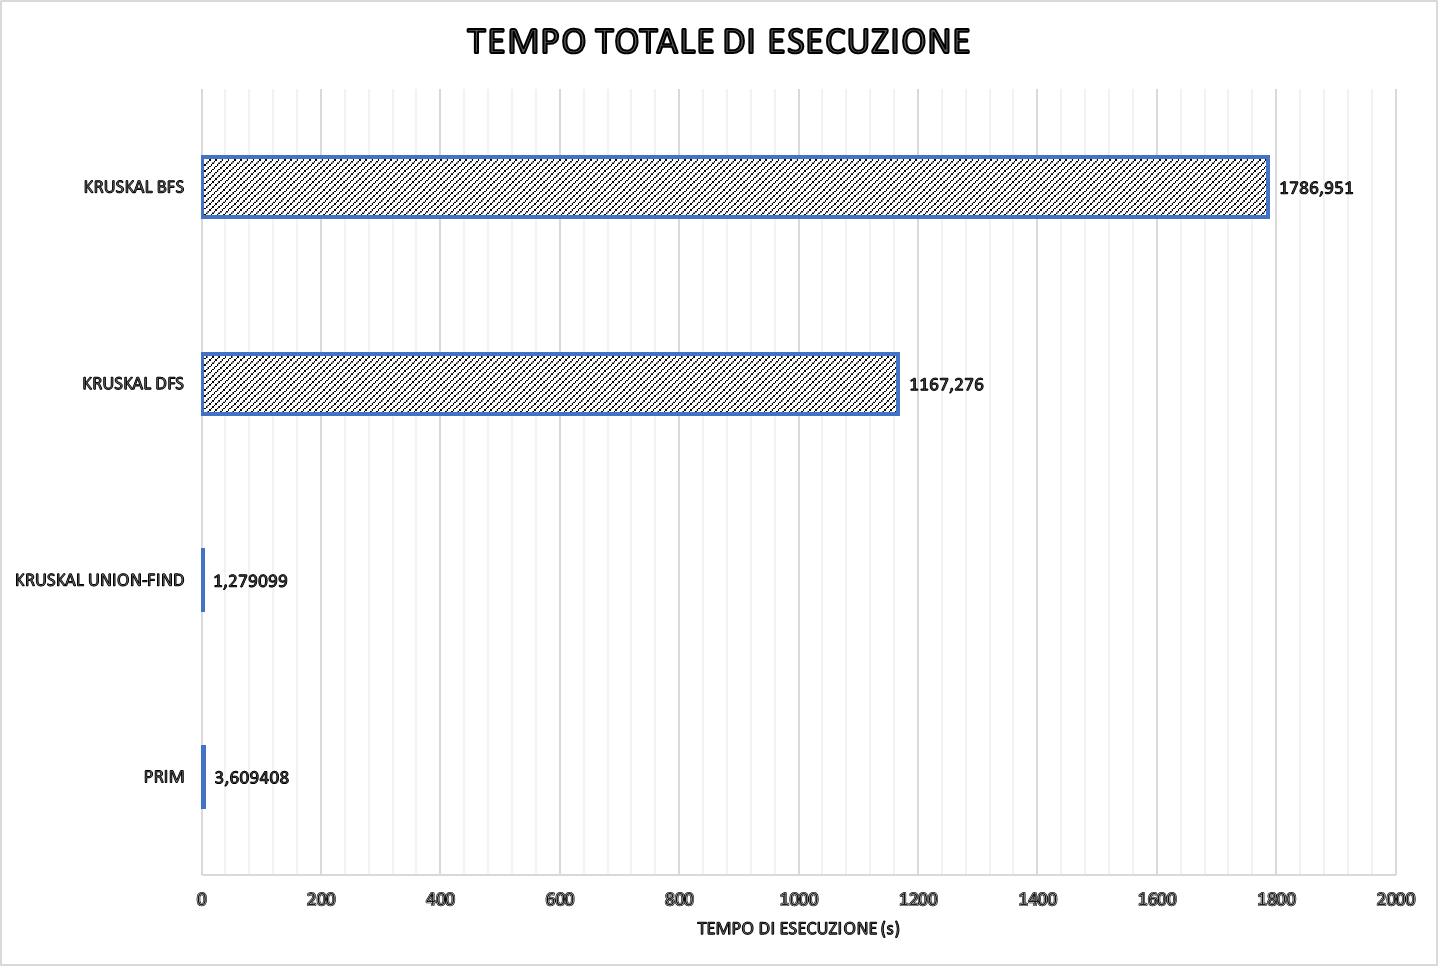
\includegraphics[width=0.8\textwidth,height=\textheight,keepaspectratio]{grafo_costo_totale.png}
	\caption{\textbf{Tempo di esecuzione totale}}
	\label{total}
\end{figure}
Considerando invece i tempi di esecuzione medi in relazione al numero di nodi di un grafo, ci accorgiamo che, per grafi di piccola taglia, le varianti DFS e BFS di Naive Kruskal risultano essere più efficienti di Prim e Kruskal Union-Find.\\
Come si può notare dalla Figura \ref{conf_tot}, Kruskal DFS e Kruskal BFS hanno tempi medi d'esecuzione più bassi rispetto agli altri algoritmi per grafi con numero di nodi, rispettivamente, minori di 200 e 100. Questo fenomeno è probabilmente dovuto all'overhead causato dall'utilizzo di strutture dati come MinHeap e Disjoint-Set che diventa tuttavia trascurabile per grafi di taglia sufficientemente alta ed è compensato dai benefici che esse forniscono in termini di efficienza.
\begin{figure}[h]
	\centering
	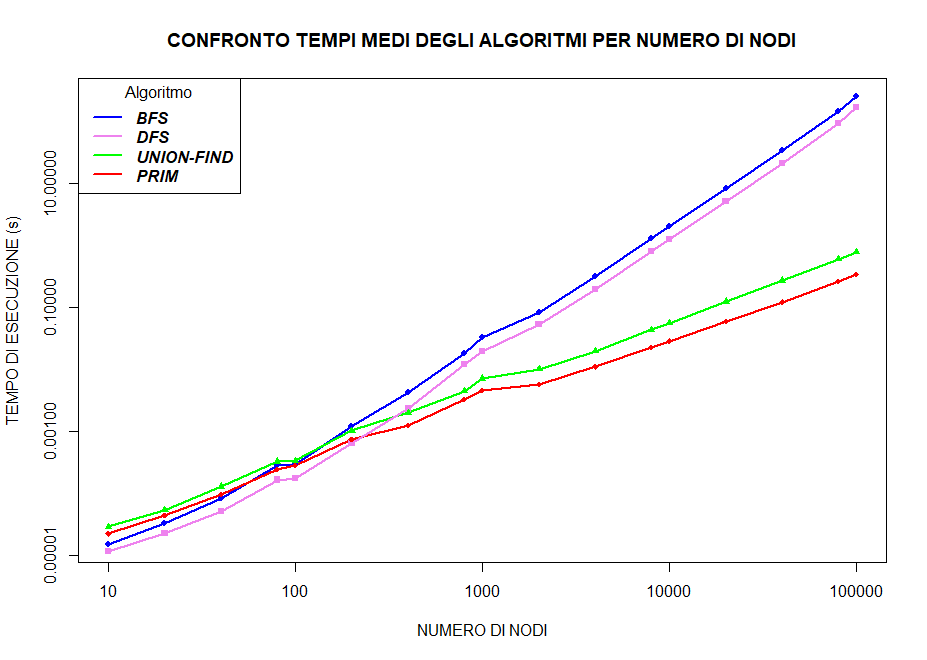
\includegraphics[width=0.9\textwidth,height=\textheight,keepaspectratio]{CONFRONTO_TOTALE.png}
	\caption{\textbf{Confronto tra algoritmi su tempi d'esecuzione medi misurati su grafi della stessa taglia}}
	\label{conf_tot}
\end{figure}

%\begin{figure}[h]
%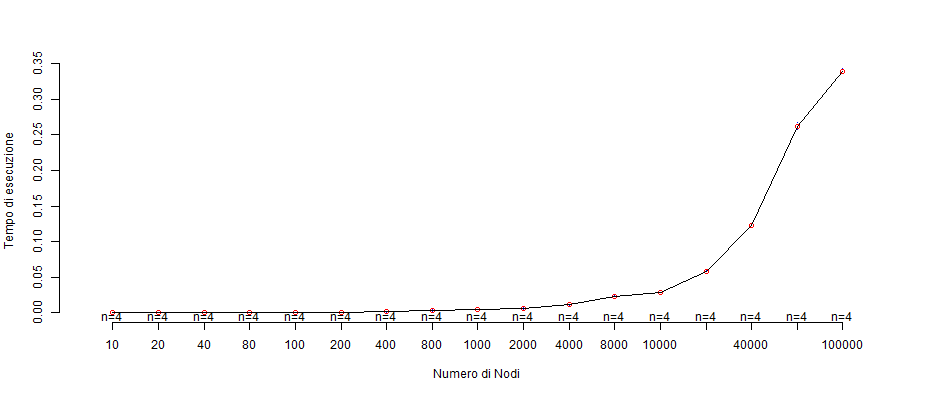
\includegraphics[width=\textwidth,height=\textheight,keepaspectratio]{PRIM_MEDIA.png}
%\caption{\textbf{PRIM}}

%possiamo osservare che prim fa robe
%\end{figure}

%\begin{figure}[h]
%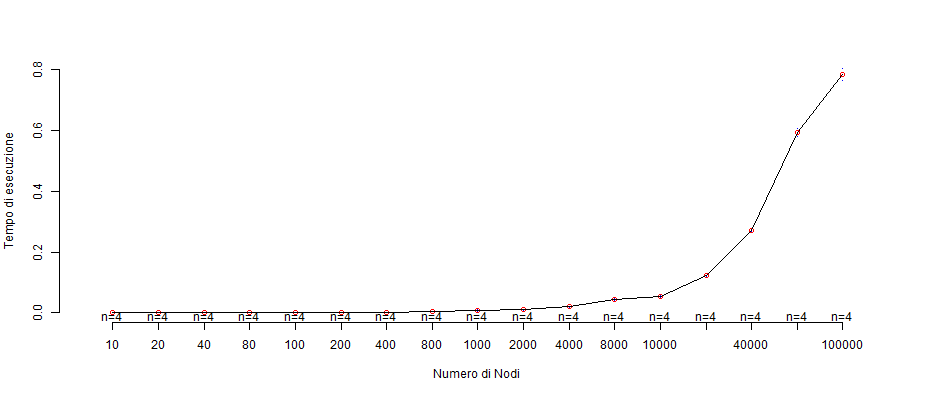
\includegraphics[width=\textwidth,height=\textheight,keepaspectratio]{K_UNION_MEDIA.png}
%\caption{\textbf{KRUSKAL UNION-FIND}}

%possiamo osservare che union find è leggermente più lento di prim
%\end{figure}

%\begin{figure}[h]

%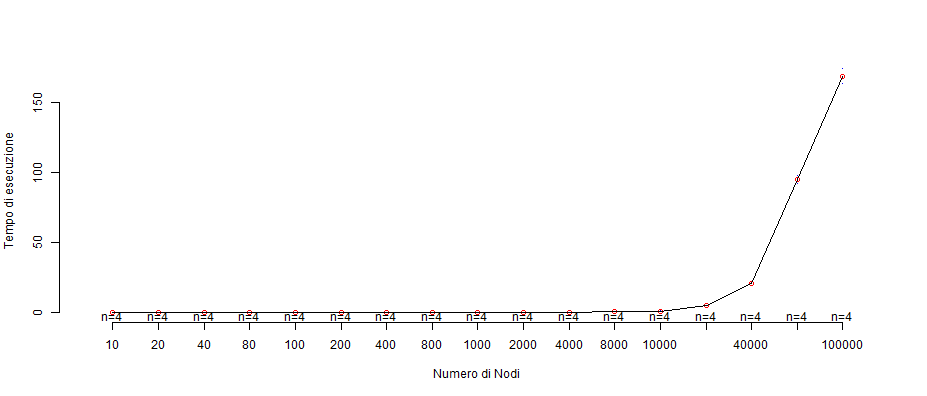
\includegraphics[width=\textwidth,height=\textheight,keepaspectratio]{K_DFS_MEDIA.png}
%\caption{\textbf{KRUSKAL DFS}}

%possiamo osservare che dfs non è molto buono
%\end{figure}

%\begin{figure}[h]

%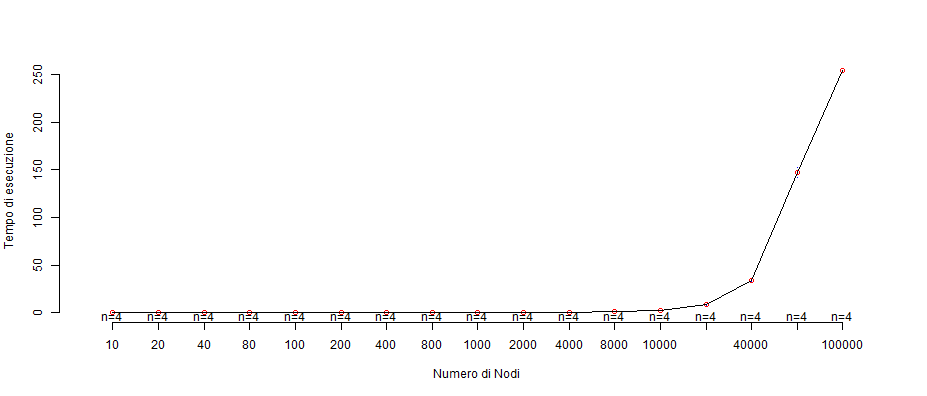
\includegraphics[width=\textwidth,height=\textheight,keepaspectratio]{K_BFS_MEDIA.png}
%\caption{\textbf{KRUSKAL BFS}}

%possiamo osservare che BFS è il peggiore
%\end{figure}
\subsubsection{Confronto tra le varianti di Naive Kruskal}
Le due varianti di Naive Kruskal differiscono unicamente nell'approccio alla \textit{cycle detection} in fase di costruzione del MST. Adottando un approccio naive al problema è possibile scegliere un qualsiasi algoritmo di ricerca su grafo per capire se tra due vertici esiste un percorso che li collega. Abbiamo perciò ritenuto interessante esplorare due possibili varianti in modo da poter scegliere la più efficiente.\\
Come mostrato in Figura \ref{dfs-bfs}, indipendentemente dalla variante selezionata, i tempi d'esecuzione sono molto simili tra loro per grafi con numero di nodi inferiore a 40.000. Tuttavia, per grafi di taglia superiore, diventa chiara la superiorità di DFS rispetto a BFS e la differenza tra i tempi di esecuzione raggiunge approssimativamente il minuto e mezzo per i grafi con 100.000 nodi.
\begin{figure}[h]
	
	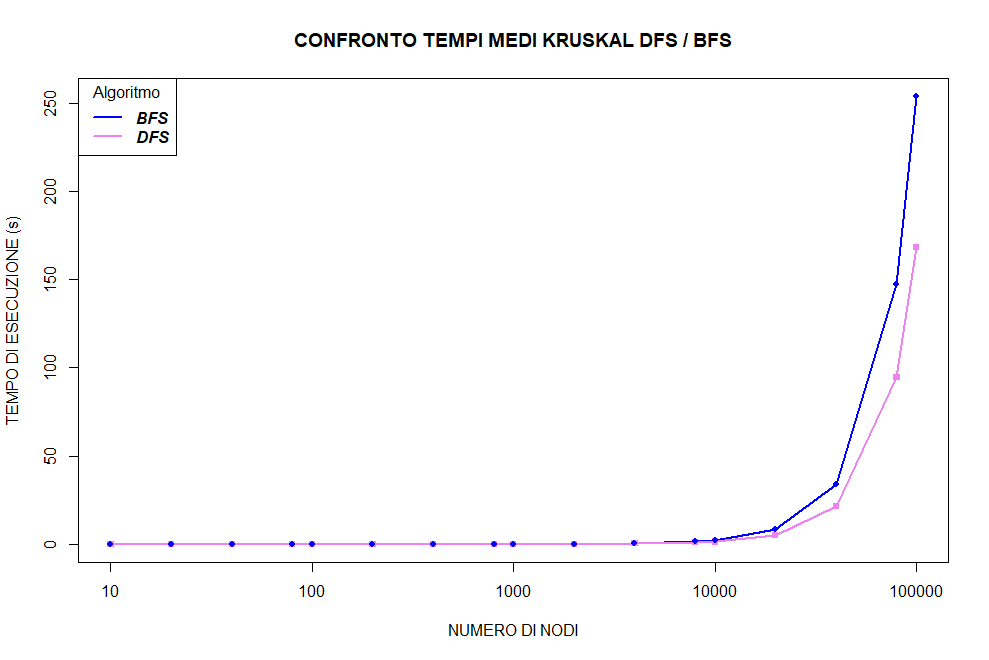
\includegraphics[width=\textwidth,height=\textheight,keepaspectratio]{COMPARE_2.png}
	\caption{\textbf{Confronto KRUSKAL DFS e BFS}}
	\label{dfs-bfs}
\end{figure}
\subsubsection{Confronto tra Prim e Kruskal Union-Find}
Sebbene, a differenza del confronto precedente, [...]
\begin{figure}[h]

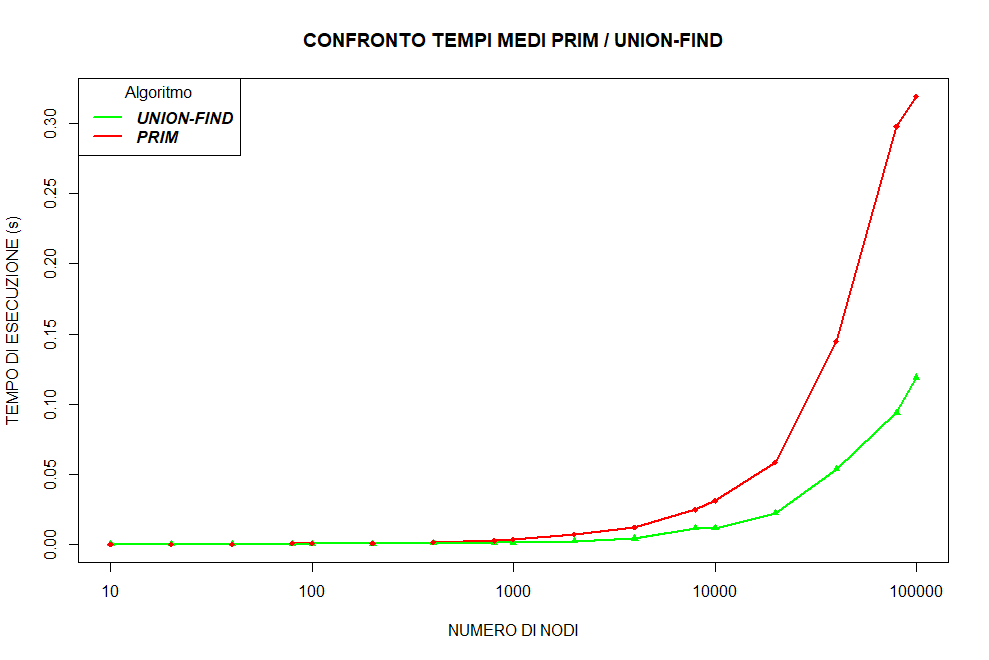
\includegraphics[width=\textwidth,height=\textheight,keepaspectratio]{COMPARE_1.png}
\caption{\textbf{Confronto PRIM e KRUSKAL Union-Find}}

All'inizio i tempi di esecuzione sono molto simili mentre intorno ai 10.000 nodi si inizia a notare una differenza nel tempo di esecuzione
\end{figure}

\end{flushleft}
\end{document}          
